\section{Belbin-Teamrollen-Test}
Mein Ergebnis des Teamrollen-Tests zeigt klar, dass ich in den Rollen des Spezialisten (13 Punkte) und des Machers (11 Punkte) besonders stark bin. Diese Rollen spiegeln nicht nur meine fachliche Tiefe wider, sondern auch meine Fähigkeit, Aufgaben direkt und entschlossen anzugehen. Als Spezialist bringe ich technisches Know-how ein und liefere Lösungen, die das Team voranbringen. Die Macher-Rolle zeigt, dass ich es bevorzuge, Verantwortung zu übernehmen und Projekte effizient abzuschließen, ohne unnötig Zeit zu verlieren.
Mit jeweils 9 Punkten in den Rollen des Neuerers/Erfinders und des Wegbereiters/Weichenstellers wird deutlich, dass ich auch kreative Ansätze verfolge. Ich bringe gerne frische Ideen ein und habe ein Gespür für strategische Lösungen, die langfristig Wirkung zeigen. Der Wert des Teamarbeiters (8 Punkte) zeigt außerdem, dass ich in der Lage bin, den Teamgeist zu fördern und eine harmonische Zusammenarbeit sicherzustellen.
Im Vergleich dazu sind die Werte für den Beobachter (4 Punkte) und den Perfektionisten (5 Punkte) niedriger. Das deutet darauf hin, dass detaillierte Analysen und eine absolute Perfektion weniger im Vordergrund stehen. Vielmehr setze ich auf pragmatisches Handeln, um schnelle und effiziente Ergebnisse zu erzielen.
Insgesamt unterstreicht das Testergebnis meine Fähigkeit, Teams aktiv zu leiten, technische Herausforderungen zu meistern und dabei auch innovative Lösungen zu entwickeln. Ich fokussiere mich darauf, Ergebnisse zu liefern, ohne dabei die Teamdynamik aus den Augen zu verlieren.

\begin{figure}[H]
	\begin{center}
		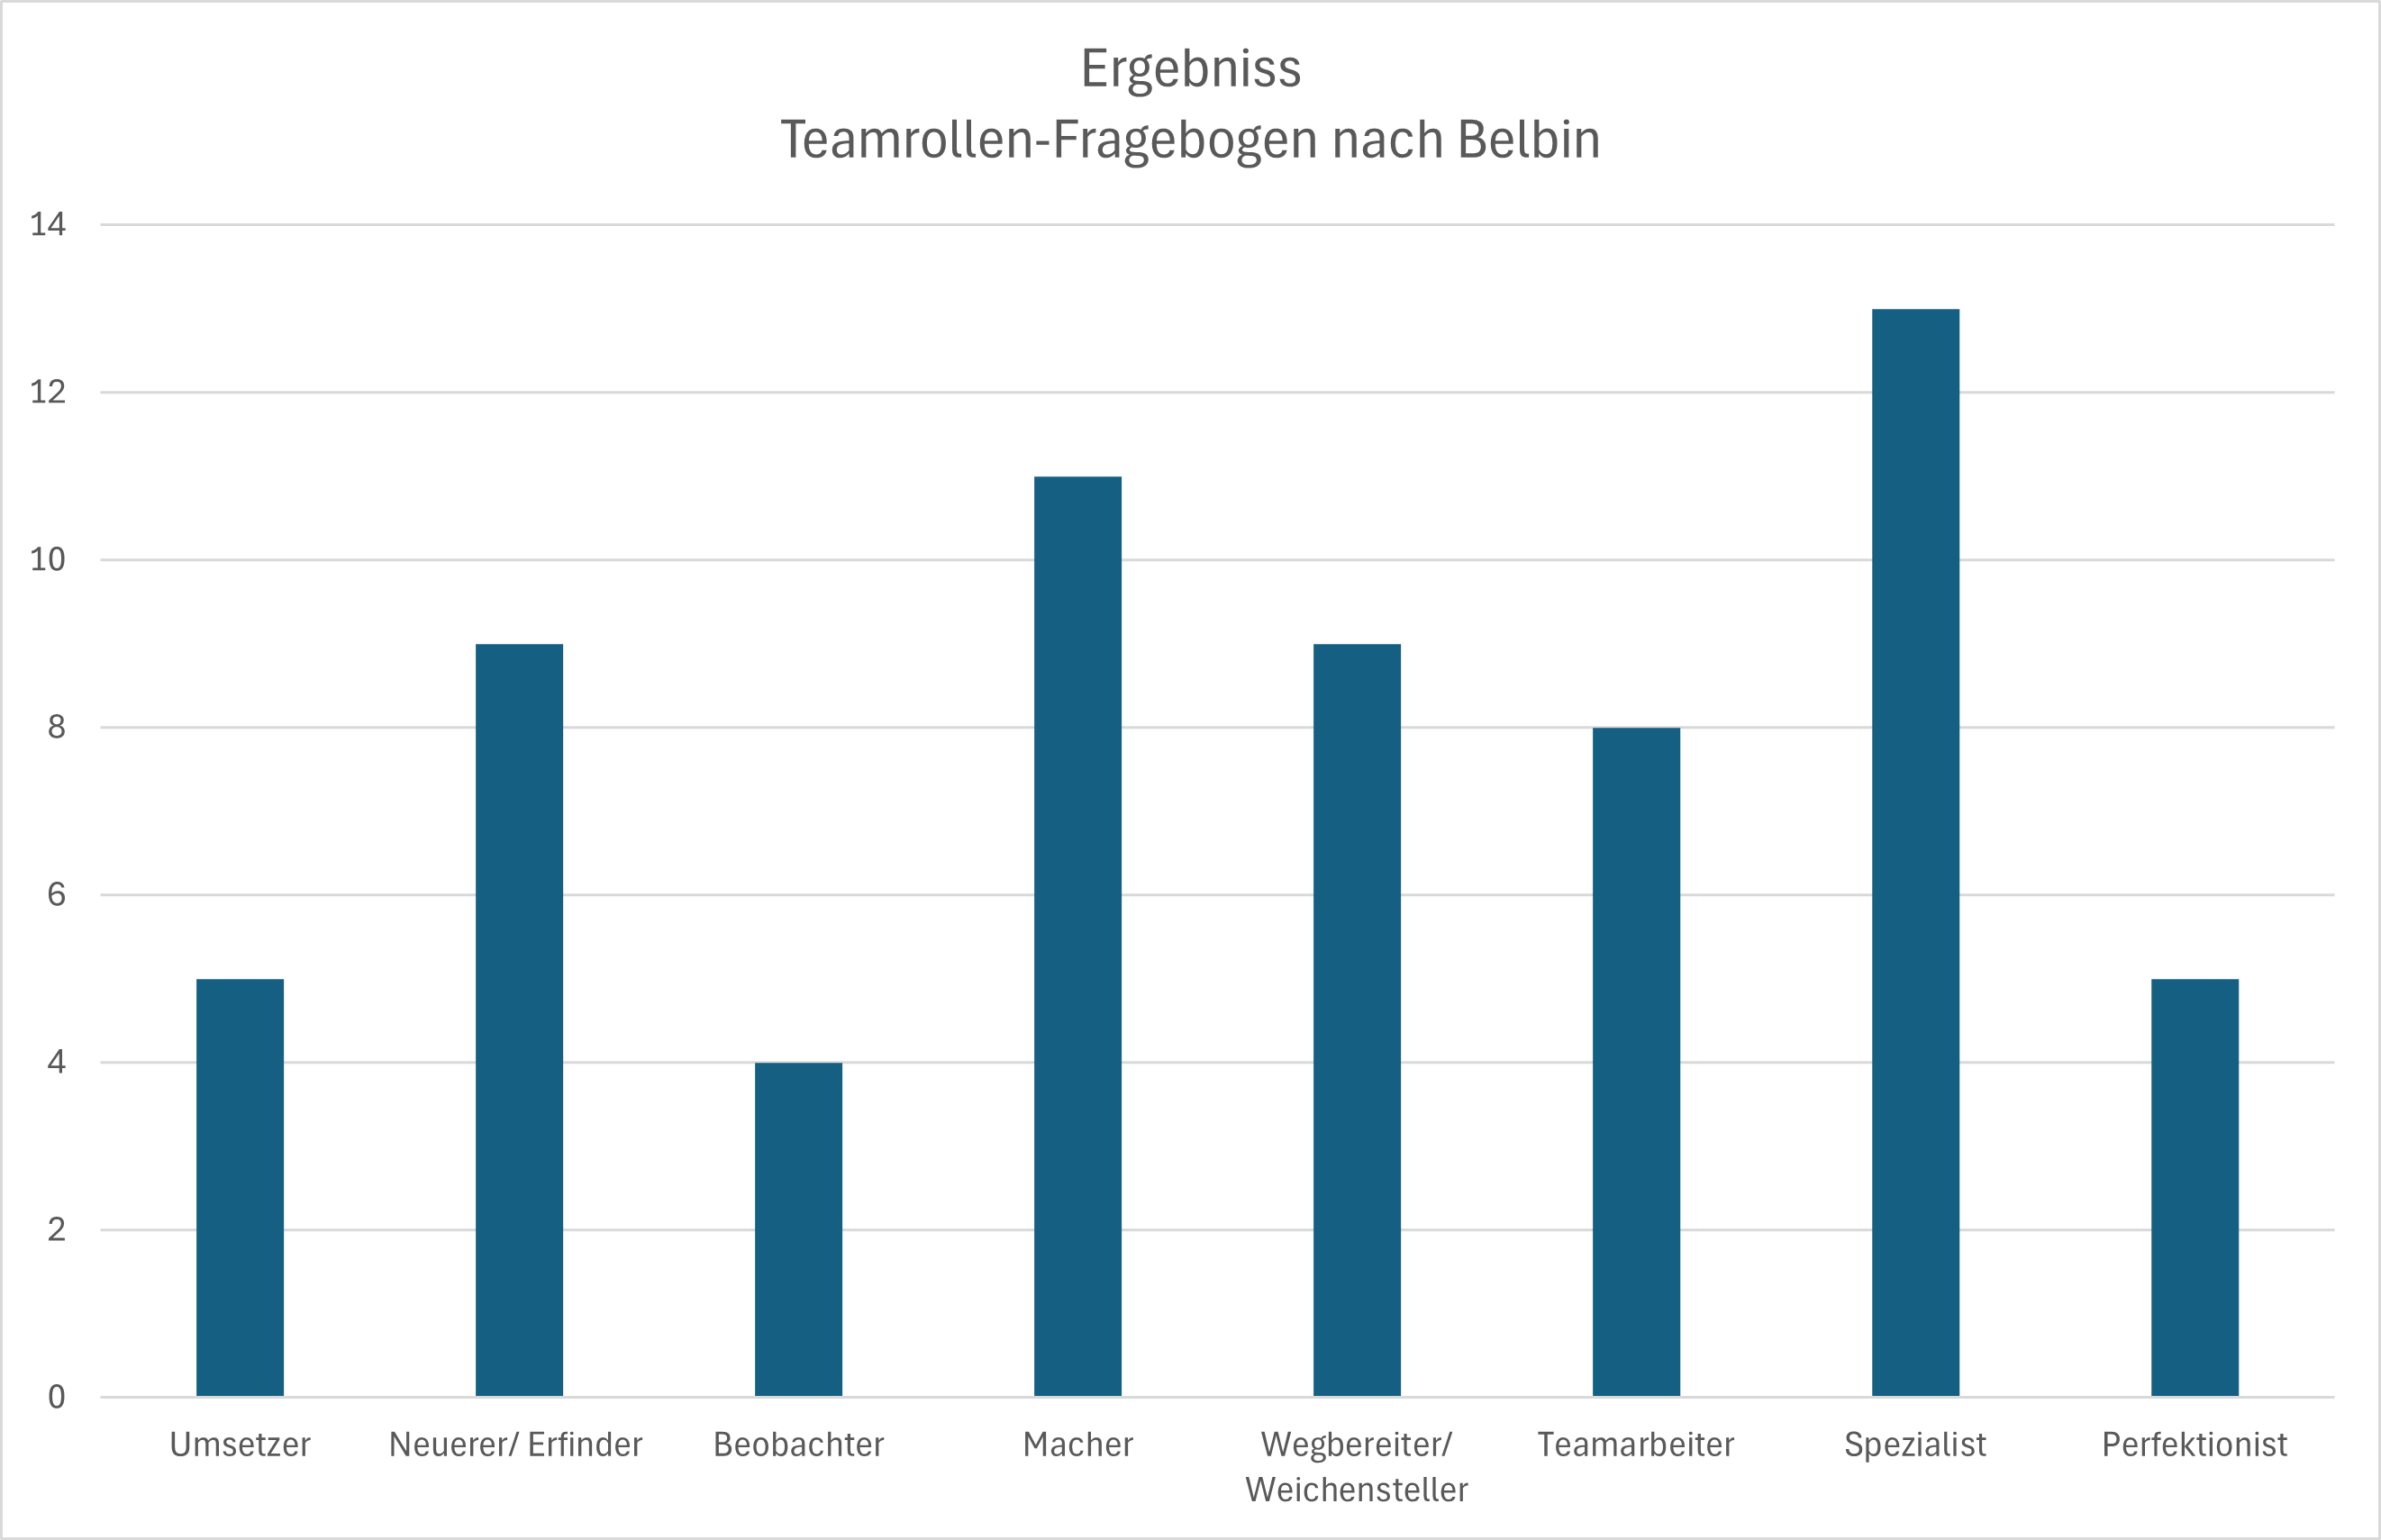
\includegraphics[width=0.8\textwidth]{Pictures/ErgebnisBelbin.png}
    \end{center}
	\caption[Ergebniss Teamrollen-Fragebogen nach Belbin]{Ergebniss Teamrollen-Fragebogen nach Belbin}
	\label{fig:ErgebnisBelbin}
\end{figure}

\newpage
